\documentclass[10pt,hyperref={CJKbookmarks=true},xcolor=dvipsnames,aspectratio=169]{beamer}
\usetheme[navigation]{UMONS}
\usepackage[utf8]{inputenc}
\usepackage{verbatim}
\usepackage{ctex}

\title[国际经济学]{国际经济学}
\subtitle{技术与贸易:李嘉图模型}
\author{鲁晓东}
\institute[]{%
	岭南学院\hspace{2em}中山大学
	\\[4ex]
	
\includegraphics[height=8ex]{fig/lingnanlogo}\hspace{2em}%
	
\includegraphics[height=8.5ex]{fig/sysu}
}
%------------section前展示一页----------
\AtBeginSection[] {     
	\begin{frame}        
	\tableofcontents[currentsection,hideallsubsections]    
\end{frame} 
}

%-------------subsection也展示一下----------
\AtBeginSubsection[]{
	
	\frame<beamer>{ 
		
		\frametitle{Outline}   
		
		\tableofcontents[currentsection,currentsubsection] 
		
	}
	
}
%---------------------------

%-----------一段一闪现-------
%\beamerdefaultoverlayspecification{<+->}
%这个功能基本不用

\begin{document}
	\maketitle
	
	
	\begin{frame}
	\frametitle{提纲}
	\tableofcontents
\end{frame}				%生成提纲页

%-----------正文开始----------------------

\section{Motivation}

\begin{frame}{Movtivation1:贸易的原因}

\begin{table}[2017年美国T恤衫进口]
	\begin{tabular}{c|c|c|c|c|c}
		\hline
		Rank                     & Expoter                         & Commodity Code                & Trade Value (US\$)                   & Netweight (kg)                    & Percentage(\%)               \\ \hline
		\textbf{0}               & \textbf{World}                  & \textbf{610910}               & \textbf{\$3,939,487,398}             & \textbf{161,316,821}              & \textbf{100}                 \\ \hline
		{\color[HTML]{FE0000} 1} & {\color[HTML]{FE0000} Honduras} & {\color[HTML]{FE0000} 610910} & {\color[HTML]{FE0000} \$541,068,929} & {\color[HTML]{FE0000} 22,156,060} & {\color[HTML]{FE0000} 13.73} \\ \hline
		2                        & Nicaragua                       & 610910                        & \$385,393,167                        & 15,781,342                        & 9.78                         \\ \hline
		3                        & El Salvador                     & 610910                        & \$370,243,245                        & 15,160,973                        & 9.40                         \\ \hline
		{\color[HTML]{3531FF} 4} & {\color[HTML]{3531FF} China}    & {\color[HTML]{3531FF} 610910} & {\color[HTML]{3531FF} \$353,089,253} & {\color[HTML]{3531FF} 14,458,539} & {\color[HTML]{3531FF} 8.96}  \\ \hline
		5                        & Dominican Rep.                  & 610910                        & \$299,211,186                        & 12,252,304                        & 7.60                         \\ \hline
		6                        & Mexico                          & 610910                        & \$291,275,395                        & 11,927,343                        & 7.39                         \\ \hline
		7                        & Haiti                           & 610910                        & \$268,398,127                        & 10,990,549                        & 6.81                         \\ \hline
		8                        & Viet Nam                        & 610910                        & \$233,827,373                        & 9,574,923                         & 5.94                         \\ \hline
		9                        & India                           & 610910                        & \$216,850,294                        & 8,879,734                         & 5.50                         \\ \hline
		10                       & Bangladesh                      & 610910                        & \$194,298,280                        & 7,956,258                         & 4.93                         \\ \hline
	\end{tabular}
\end{table}
  \begin{itemize}
  	\item 美国完全拥有制造T恤衫的技术,为什么还要从洪都拉斯进口?
  	\item 中国的纺织品生产技术是全球最高的,为什么美国还从技术落后的洪都拉斯等国进口?
  \end{itemize}
\end{frame}


\begin{frame}{Motivation2:如何看待国家之间的经济catchup}


\begin{columns}[onlytextwidth]
	\begin{column}{0.4\textwidth}
		\begin{itemize}
			\item 2018年,中美贸易战发生的直接导火索是什么?
			\item Some foreign economies have been growing much faster than U.S. 
			\item Partly due to population growth but also due to technological catch
			-up
		\end{itemize}
		
	\end{column}
	\begin{column}{0.6\textwidth}
\begin{figure}
	\centering
	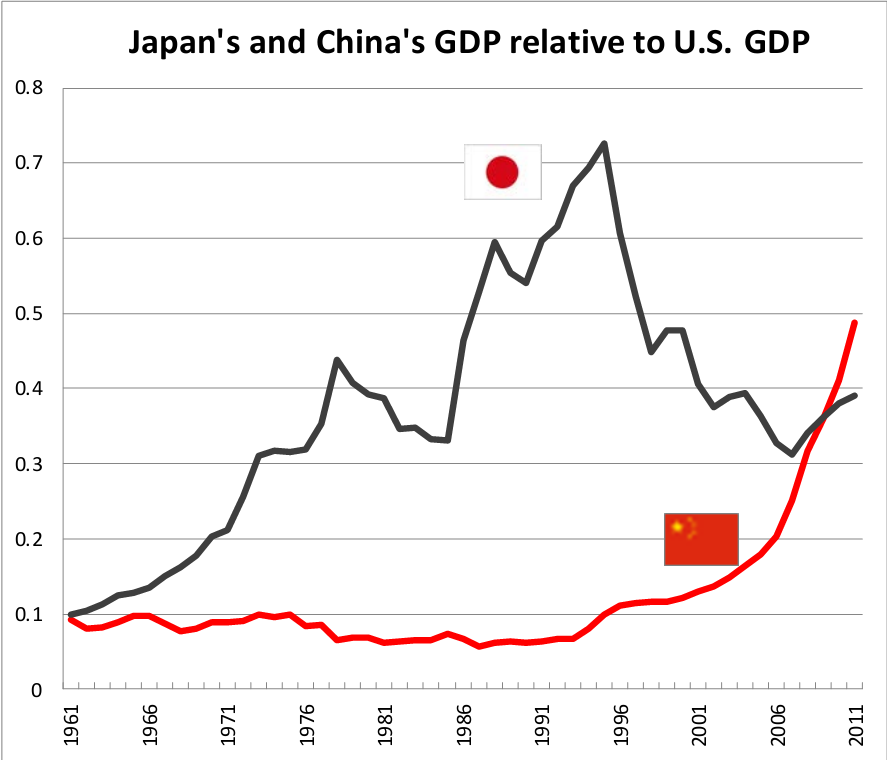
\includegraphics[width=0.7\linewidth]{fig/ricardo/lec3-00}

\end{figure}
	\end{column}
\end{columns}

\end{frame}

\begin{frame}{Some Reactions }


\begin{figure}

\centering{}
\includegraphics[width=6cm]{fig/ricardo/lec3-010}
\centering{}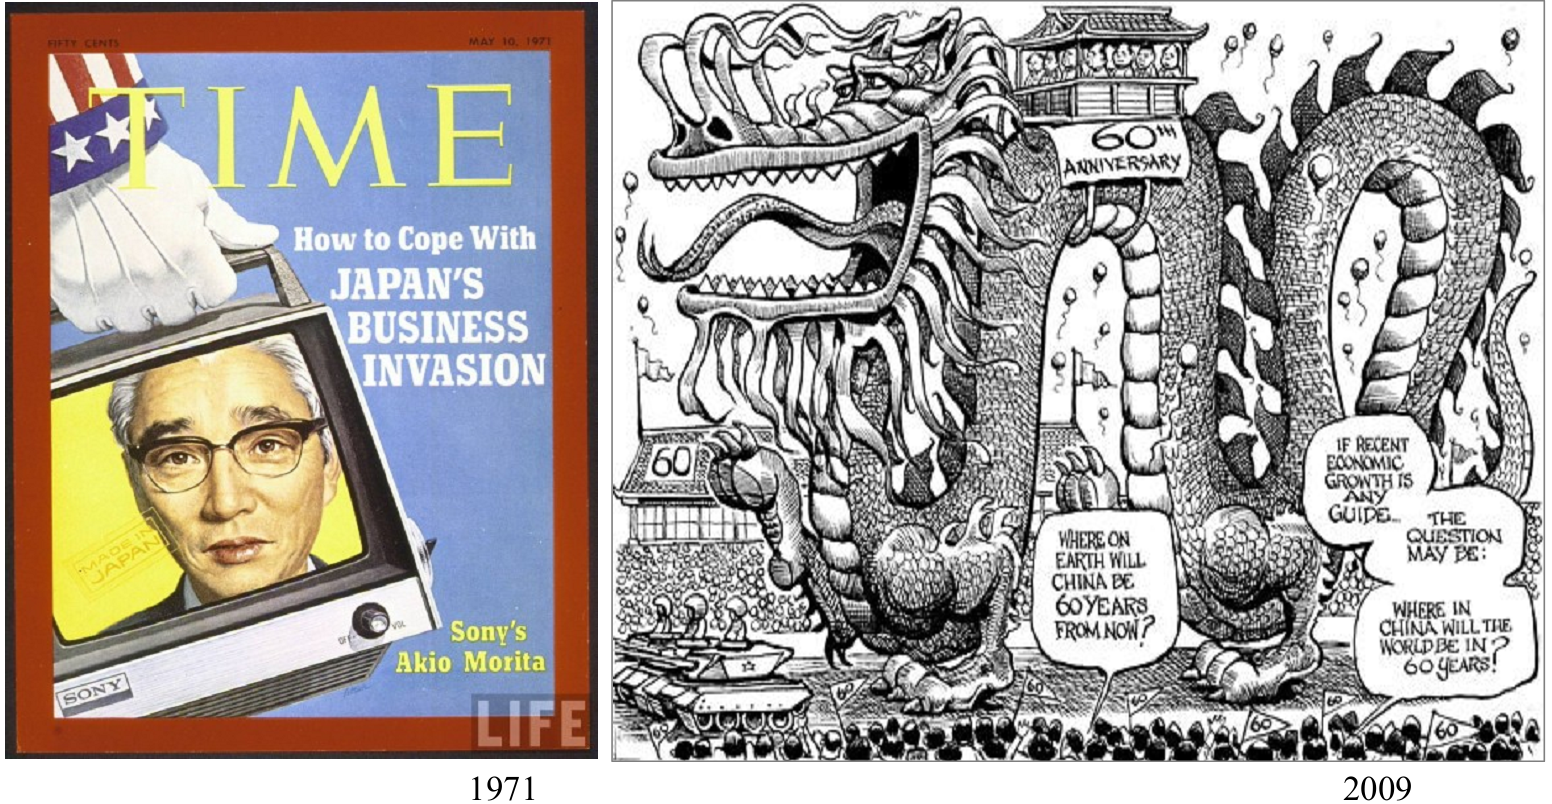
\includegraphics[width=10cm]{fig/ricardo/lec3-01}
\end{figure}

\end{frame}

\begin{frame}{Enter the Ricardian Model }

\begin{itemize}
\item Are these reactions justified? 
\item What is the effect of growth abroad on the U.S. economy? 
\item 面对其他国家的技术赶超,何种态度才是符合理性精神的? 
 
\item The Ricardian model provides the most widely used model to think about
these issues conceptually
\end{itemize}
\end{frame}

\section{Ricardo's Insight}
\begin{frame}{Gains from Trade: An Obvious Example}

\begin{itemize}
\item Imagine a world with two countries (England and Portugal) producing
and consuming two goods (cloth and wine) 
\item There are 100 workers in each country 
\item If England allocates all of its workers to producing… 

\begin{itemize}
\item \textcolor{red}{\uline{cloth}}, they can produce 1,000 pieces of
cloth 
\item \textcolor{red}{\uline{wine}} , they can produce 500 bottles of
wine 
\end{itemize}
\item If Portugal allocates all of its workers to producing… 

\begin{itemize}
\item \textcolor{red}{\uline{cloth}}, they can produce 500 pieces of
cloth 
\item \textcolor{red}{\uline{wine}} , they can produce 1,000 bottles
of wine 
\end{itemize}
\end{itemize}
\end{frame}

\begin{frame}{Autarky Equilibrium }

\begin{itemize}
\item Consider an autarky equilibrium where countries can only consume what
they produce 
\item Assume that 60 workers are employed in cloth production, 40 in wine
production
\item Then, England produces (and consumes) 600 pieces of cloth and 200
bottles of wine 
\item Portugal produces 300 pieces of cloth and 400 bottles of wine 
\item \uline{“World” jointly produces (and consumes) 900 pieces of cloth
and 600 bottles of wine }
\end{itemize}
\end{frame}

\begin{frame}{Free Trade Equilibrium }

\begin{itemize}
\item Suppose now that England and Portugal can freely trade across borders
\item Suppose England produces only cloth and Portugal only wine 
\item World now jointly produces 1,000 pieces of cloth and 1,000 bottles
of wine 
\item So world consumption goes up. There are \structure<+->{overall gains} from trade 

\item How are gains \textcolor{red}{distributed} within and across countries?
Less clear: we need \textbf{\textcolor{red}{a model}} to determine
prices
\end{itemize}
\end{frame}

\begin{frame}{A Way to Determinate Labor Division}
\begin{columns}
  \begin{column}{0.6\textwidth}


\begin{itemize}
\item The Production Possibility of the two countries
\end{itemize}

\begin{center}
\begin{tabular}{|c|c|c|}
\hline 
& Cloth & Wine\tabularnewline
\hline 
\hline 
England & 1000 & 500\tabularnewline
\hline 
Portugal & 500 & 1000\tabularnewline
\hline 
\end{tabular}
\par\end{center}
\begin{itemize}
\item The Labor Productivity ($Q_{i}/L_{i}$) of the two countries 
\end{itemize}

\pause{}


\begin{center}
\begin{tabular}{|c|c|c|}
\hline 
& Cloth & Wine\tabularnewline
\hline 
\hline 
England & \textbf{\textcolor{red}{10}} & 5\tabularnewline
\hline 
Portugal & 5 & \textbf{\textcolor{red}{10}}\tabularnewline
\hline 
\end{tabular}
\par\end{center}
\begin{itemize}
\item The Production Cost of the two countries
\end{itemize}

\pause{}


\begin{center}
\begin{tabular}{|c|c|c|}
\hline 
& Cloth & Wine\tabularnewline
\hline 
\hline 
England & 0.1 & \textbf{\textcolor{red}{0.2}}\tabularnewline
\hline 
Portugal & \textbf{\textcolor{red}{0.2}} & 0.1\tabularnewline
\hline 
\end{tabular}
\par\end{center}
\end{column} 
 \begin{column}{0.4\textwidth}

\begin{itemize}
\item This is the Adam Smith's intelligence! We called it \textbf{\textcolor{red}{Absolute
Advantage}}
\end{itemize}
\end{column}
\end{columns}
\end{frame}

\begin{frame}{从绝对优势到比较优势:A Less Obvious Example}

\begin{itemize}
\item The previous example was obvious because England had absolute advantage
in producing cloth, while Portugal had absolute advantage in producing
wine 
\item Suppose now that Portugal can only produce a maximum of 600 pieces
of cloth and 400 bottles of wine 
\item The Production Possibility of the two countries
\end{itemize}

\begin{center}
\begin{tabular}{|c|c|c|}
\hline 
& Cloth & Wine\tabularnewline
\hline 
\hline 
England & 1000 & 500\tabularnewline
\hline 
Portugal & 600 & 400\tabularnewline
\hline 
\end{tabular}
\par\end{center}
\begin{itemize}
\item England has \textbf{\textcolor{red}{Absolute Advantage}} in both goods.
Does it pay for England to trade with Portugal? 
\end{itemize}
\end{frame}

\begin{frame}{An Intuitive But Wrong Answer }

\begin{itemize}
\item England should not buy cloth or wine from Portugal because English
“firms” are more productive than Portuguese “firms” 
\item Related modern examples (or misconceptions): 

\begin{itemize}
\item Less - developed economies should not follow free trade practices
because these countries are not “competitive” enough 
\item U.S. firms must keep their competitive edge unless they want to be
wiped out from world markets
\end{itemize}
\end{itemize}
\end{frame}

\begin{frame}{Ricardo’s Insight }

\begin{itemize}
\item Suppose that autarky production in England is as before (600 pieces
of cloth and 200 bottles of wine) 
\item Portugal now produces 600 x 0.6 = 360 pieces of cloth and 400 x 0.4
= 160 bottles of wine (maintain 60/40 distribution of workers) 
\item So World now produces 960 pieces of cloth and 360 bottles of wine
under autarky 
\item What happens when England produces only cloth and Portugal only wine
and there is free trade? 
\end{itemize}
\end{frame}

\begin{frame}{Ricardo’s Insight (cted.) }

\begin{itemize}
\item World now produces 1,000 pieces of cloth and 400 bottles of wine 
\item Again there are aggregate gains from trade! 
\item \textcolor{red}{Possible }Equilibrium: 

\begin{itemize}
\item England consumes 600 pieces of cloth and 240 bottles of wine 
\item Portugal consumes 400 pieces of cloth and 160 bottles of wine 
\end{itemize}
\item So both countries gain from trade! 
\end{itemize}
\end{frame}

\begin{frame}[allowframebreaks]{Comparative Advantage}

\begin{itemize}
\item Countries generally find it beneficial to specialize in the production
of goods that they can produce relatively (or comparatively) more
efficiently
\item England can produce cloth and wine more efficiently, but the advantage
is relatively higher in cloth (1,000/600 > 500/400) 
\item Paul Samuelson: “comparative advantage is the best example of a proposition
in all of the social sciences which is both true and non- trivial” 
\item The ways to measure comparative advantage

\begin{itemize}
\item Relative labor productivity
\item Relatvie labor cost
\item Opportunity cost

\begin{itemize}
\item the opportunity cost of producing something measures the cost of not
being able to produce something else 
\end{itemize}
\end{itemize}
\item \textcolor{blue}{\uline{Definition: A country has a comparative
advantage in producing a good if the opportunity cost of producing
the good in that country is lower than it is in other countries }}
\end{itemize}
\end{frame}

\begin{frame}{Measurement of Comparative Advantage}

\begin{itemize}
\item Relative labor productivity
\end{itemize}

\pause{}


\begin{center}
\begin{tabular}{|c|c|c|}
\hline 
& Cloth/Wine & Wine/Cloth\tabularnewline
\hline 
\hline 
England & \textbf{\textcolor{red}{2}} & 0.5\tabularnewline
\hline 
Portugal & 1.5 & \textbf{\textcolor{red}{0.66}}\tabularnewline
\hline 
\end{tabular}
\par\end{center}
\begin{itemize}
\item Relatvie labor cost
\end{itemize}

\pause{}


\begin{center}
\begin{tabular}{|c|c|c|}
\hline 
& Cloth/Wine & Wine/Cloth\tabularnewline
\hline 
\hline 
England & \textbf{\textcolor{red}{0.5}} & 2\tabularnewline
\hline 
Portugal & 0.66 & \textbf{\textcolor{red}{1.5}}\tabularnewline
\hline 
\end{tabular}
\par\end{center}
\begin{itemize}
\item Opportunity cost
\end{itemize}

\pause{}


\begin{center}
\begin{tabular}{|c|c|c|}
\hline 
& Cloth & Wine\tabularnewline
\hline 
\hline 
England & \textbf{\textcolor{red}{(1/10){*}5=0.5 wine}} & (1/5){*}10=2 Cloth\tabularnewline
\hline 
Portugal & (1/6){*}4=0.66 wine & \textbf{\textcolor{red}{(1/4){*}6=1.5 cloth}}\tabularnewline
\hline 
\end{tabular}
\par\end{center}


\end{frame}

\begin{frame}{David Ricardo }




\begin{columns}[onlytextwidth]
\begin{column}{0.6\textwidth}
\begin{itemize}
\item Concept of comparative advantage first proposed by David Ricardo (1772-1823) 
\item The richest economist in history

\begin{itemize}
\item made £1,000,000 in waterloo battle
\end{itemize}
\item May be the first economist discriminate female and leave a bad tradition
in economic field
\begin{block}{对比较优势理论的评价}
	比较优势是这样一个最佳的例子,即一个经济学原理无疑是正确的,但是对于聪明的人而言却并非显而易见的。\\
		\textcolor{blue}{————萨缪尔森《一个经济学家的道路》}
\end{block}
\end{itemize}

\end{column}
\begin{column}{0.4\textwidth}
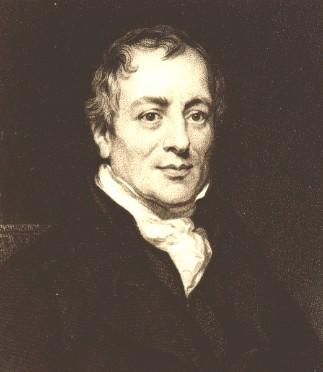
\includegraphics[scale=0.5]{fig/ricardo/lec3-03}
\end{column}
\end{columns}




\end{frame}



\section{A Formal Ricardian Model}
\begin{frame}{A Formal Ricardian Model }

	\begin{block}{脑洞题}
		你们都学过经济学原理,经济学原理中最基础的模型就是市场模型,市场模型里的价格是有什么因素决定的?你是否能想出一种情形,在这种情形下,价格由单一方面决定?
	\end{block}
\begin{itemize}
\item Two -country world with a Home country and a Foreign one 
\item Labor is the only factor of production and is in fixed supply 
\item Only two goods are relevant for production and consumption (wine and
cloth) 
\item Labor productivity varies across countries and goods (due to differences
in technology) 
\item Labor can move freely across sectors 
\item There are constant returns to scale, so technology can be summarized
by a unique number for each good and country 
\item All markets are competitive so that wine and cloth producers take
prices and wages as given 
\end{itemize}
\end{frame}

\begin{frame}{Unit Labor Requirements }

\begin{itemize}
\item Because labor productivity is constant, we can define a \textcolor{blue}{\uline{unit
labor requirement}} as the constant number of units of labor required
to produce one unit of output 
\item $a_{LW}$ is the unit labor requirement for wine in the Home country 

\begin{itemize}
\item this implies that 1 unit of labor (say 1 worker) produces $1/a_{LW}$
units (say bottles) of wine 
\end{itemize}
\item $a_{LC}$is the unit labor requirement for cloth in the Home country 
\item $a*_{LC}$and $a*_{LW}$ are the analogous numbers for the Foreign
country 
\item A high unit labor requirement hence implies a low labor productivity
level
\end{itemize}
\end{frame}

\begin{frame}{Production Possibility Frontier}


The production possibility frontier (PPF) of an economy represents
the maximum amount of goods that can be produced from a fixed amount
of resources 

For the Home economy, we can write this as the combination of $Q_{C}$
and $Q_{W}$ such that 

\begin{figure}


\centering{}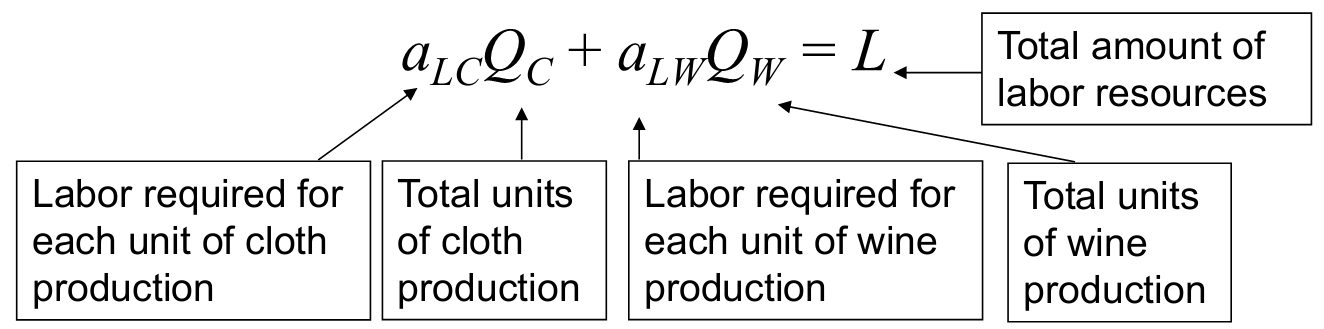
\includegraphics[width=12cm]{fig/ricardo/lec3-04}
\end{figure}

\end{frame}

\begin{frame}{A Graph of the PPF}


\begin{columns}[onlytextwidth]
\begin{column}{0.4\textwidth}
\begin{itemize}
\item With only one factor of production and constant returns to scale,
the PPF is linear in the space ($Q_{C}$ ,$Q_{W}$ ) 
\item The slope is given by ${–}(a_{LC}/a_{LW})$ 
\item Slope measures opportunity cost of cloth in terms of wine
\end{itemize}

\end{column}
\begin{column}{0.6\textwidth}
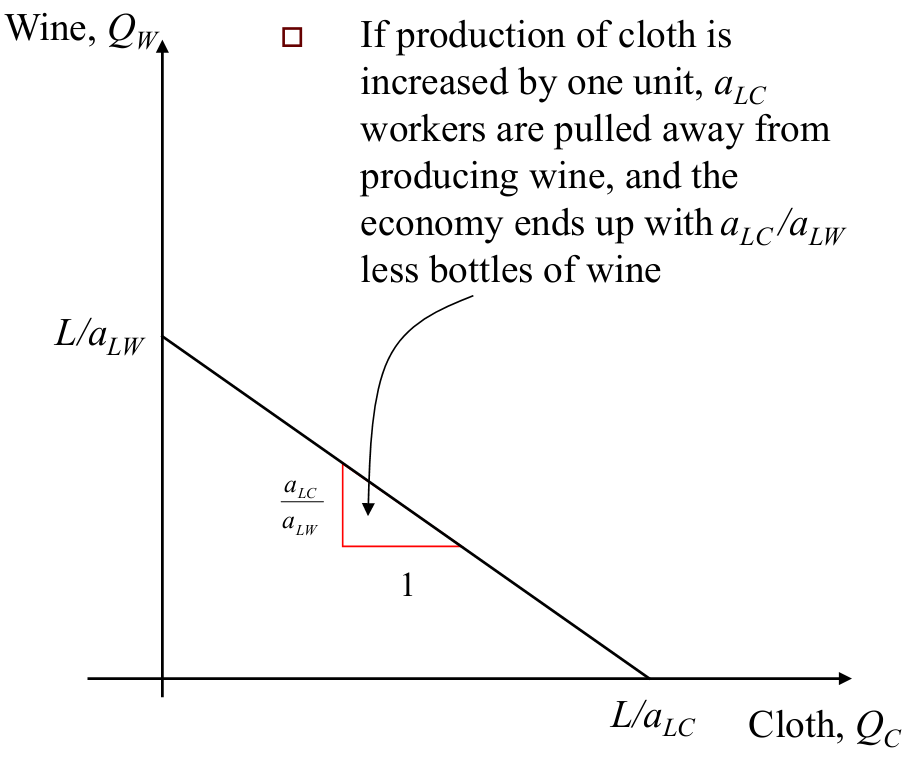
\includegraphics[width=0.8\columnwidth]{fig/ricardo/lec3-05}
\end{column}
\end{columns}

\end{frame}

\begin{frame}{Autarkic Equilibrium}

\begin{itemize}
\item So far we have discussed what an economy can produce, but 

\begin{itemize}
\item what will the economy actually produce? 
\item what will the equilibrium wage be? 
\item what will the equilibrium relative price of cloth be? 
\end{itemize}
\item Consider the profit maximization problem of firms in the cloth sector,
that is:

\begin{itemize}
\item choose $Q_{C}$ to maximize $P_{C}Q_{C}{–}wa_{LC}Q_{C}$ 
\end{itemize}
\item If $P_{C}>wa_{LC}$, firms would want to set $Q_{C}$ = +∞ (not an
equilibrium) 
\item If $P_{C}<wa_{LC}$ , firms would want to set $Q_{C}$ = 0 (not an
equilibrium if consumers “cannot live” without cloth) 
\end{itemize}
\end{frame}

\begin{frame}{Autarkic Equilibrium (cont.) }


Hence, the only prices consistent with equilibrium are 
\[
P_{C}=wa_{LC}
\]
\[
P_{W}=wa_{LW}
\]


So relative prices are such that $P_{C}/P_{W}=a_{LC}/a_{LW}$

Alternative derivation: 

because labor is the only factor of production, each worker receives$P_{C}/a_{LC}$
if employed in clothing, $P_{W}/a_{LW}$ if employed in wine production 

Only when these two numbers are equal will workers want to produce
both goods 

\textcolor{blue}{\uline{Important: with free trade, we may have
$P_{C}/P_{W}\neq a_{LC}/a_{LW}$}}
\end{frame}

\begin{frame}{Prices and Wages: Digression }

\begin{itemize}
\item Hence, we have 2 equations determining 3 prices, but remember that
we can always set one price at an arbitrary constant (e.g., 1) 

\begin{itemize}
\item If we multiply all prices and wages by a common factor, this has no
effect on firm behavior or consumer behavior 
\end{itemize}
\item The Ricardian model is special because prices are uniquely pinned
down by the supply - side of the model 
\item 问题:Ricardo 是如何做到这一点的?
\begin{itemize}
\item labor-theory of value (classical economics) 
\item generally, the demand -side of the economy will also affect value
(neoclassical economics) 
\end{itemize}
\item What the demand-side of the model determines here is the equilibrium
quantities $Q_{C}$ and $Q_{W}$ 
\end{itemize}
\end{frame}

\begin{frame}{Graphical Illustration of Equilibrium}


\begin{columns}[onlytextwidth]
\begin{column}{0.4\textwidth}
\begin{itemize}
\item The only relative price consistent with equilibrium is $a_{LC}/a_{LW}$
\item Relative demand determines the equilibrium relative production levels
\end{itemize}

\end{column}
\begin{column}{0.6\textwidth}
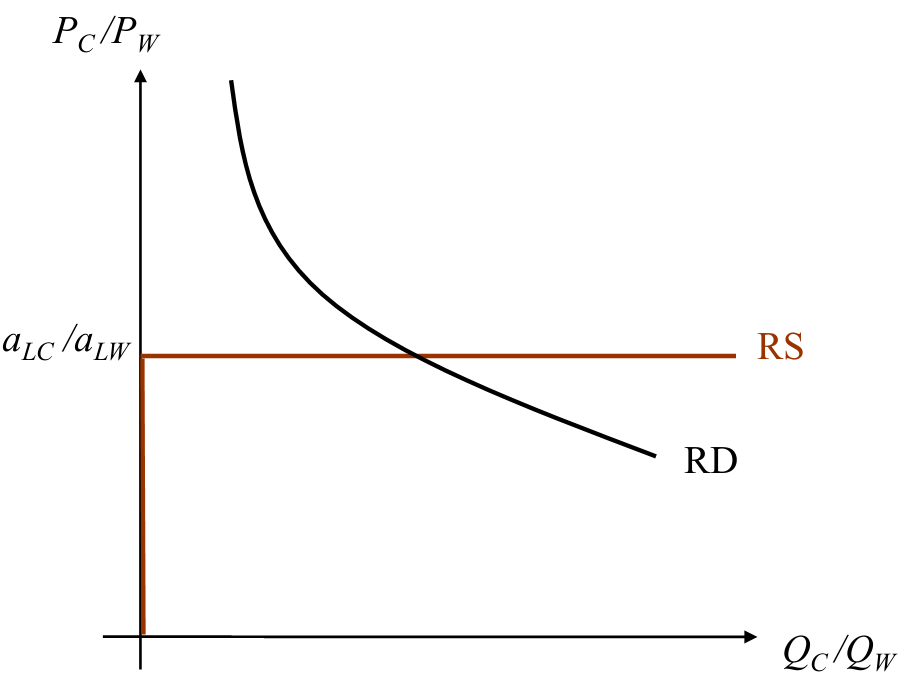
\includegraphics[width=\columnwidth]{fig/ricardo/lec3-06}
\end{column}
\end{columns}

\end{frame}

\begin{frame}{Trade in the Ricardian Model }

\begin{itemize}
\item Consider now a situation where Home and Foreign are allowed to trade
clothing and wine with each other 
\item Assume that the Foreign labor force is equal to L {*} and that unit
labor requirements in both countries satisfy 
\[
a_{LC}/a_{LW}<a{}_{LC}^{*}/a_{LW}^{*}
\]

\item This implies that under autarky: 

\begin{enumerate}
\item The opportunity cost of cloth in terms of wine is lower at Home than
in Foreign 
\item The relative price of cloth in terms of wine is lower at Home than
in Foreign 
\end{enumerate}
\item This implies that we are assuming that \textcolor{blue}{\uline{Home
has comparative advantage in cloth }}

\begin{itemize}
\item Satisfies both “relative price” and “opportunity cost” definitions
of comparative advantage 
\end{itemize}
\end{itemize}
\end{frame}

\begin{frame}{World Equilibrium }

\begin{itemize}
\item In the free trade equilibrium, we will have that: 

\begin{enumerate}
\item consumers choose their demand of cloth and wine to maximize their
utility;
\item firms choose their production levels to maximize profits; 
\item world demand and supply of each good are equated; 
\item each country’s demand and supply of labor are equated 
\end{enumerate}
\item Main difference with autarky equilibrium is part (3), where under
autarky we imposed equilibrium \textcolor{blue}{\uline{in each
country}} 
\end{itemize}
\end{frame}

\begin{frame}{Profit Maximization}

\begin{itemize}
\item Firm behavior is essentially identical to that in the autarkic equilibrium 
\item If $P_{C}/P_{W}<a_{LC}/a_{LW}<a{}_{LC}^{*}/a_{LW}^{*}$ then no firm
or worker in either country would want to produce clothing 
\item If $P_{C}/P_{W}>a_{LC}^{*}/a_{LW}^{*}>a_{LC}/a_{LW}$ then no firm
or worker in either country would want to produce wine 
\item What happens when $P_{C}/P_{W}=a{}_{LC}^{*}/a_{LW}^{*}$ or $P_{C}/P_{W}=a_{LC}/a_{LW}$
?

\begin{itemize}
\item Firms/workers in 1 country are indifferent between producing either
good 
\end{itemize}
\item What happens when $a_{LC}^{*}/a_{LW}^{*}>P_{C}/P_{W}>a_{LC}/a_{LW}$
? 

\begin{itemize}
\item Home only wants to produce cloth: $Q_{C}=L/a_{LC}$ ,$Q_{W}=0$
\item Foreign only wants to produce wine: $Q_{C}=0$, $Q_{W}^{*}=L^{*}/a_{LW}^{*}$ 
\end{itemize}
\end{itemize}
\end{frame}

\begin{frame}{World Relative Supply}


\begin{figure}
\begin{centering}
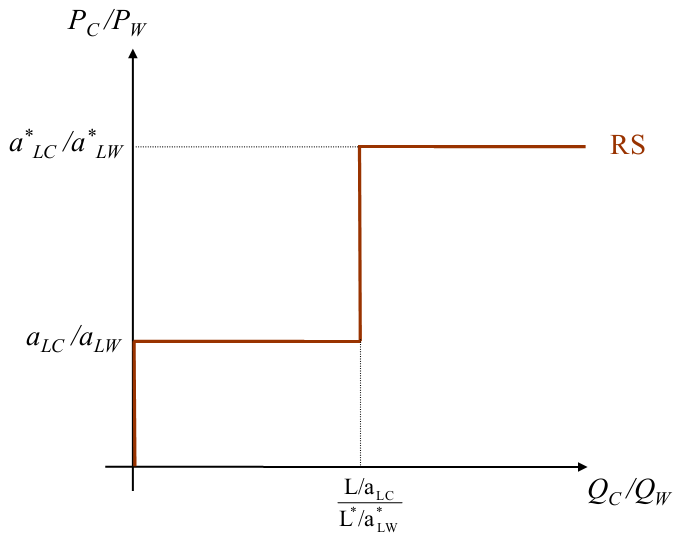
\includegraphics[width=8cm]{fig/ricardo/lec3-07}
\par\end{centering}

\end{figure}

\end{frame}

\begin{frame}{Demand Side of the Model }

\begin{itemize}
\item Up to now we have ignored the demand side of the model 

\begin{itemize}
\item It did not play any role in determining relative prices under autarky 
\end{itemize}
\item Workers receive their wage w or w {*} and they spend it on clothing
and food 
\item Assume that workers in both countries have identical homothetic preferences 

\begin{itemize}
\item This implies that their relative demand of the two goods is\textcolor{blue}{\uline{
independent of wages }}
\end{itemize}
\item Hence, the relative demand schedule is identical in both countries 
\item And since consumers in both countries face the same relative prices,
they will also have a common relative demand 
\end{itemize}
\end{frame}

\begin{frame}{World Equilibrium}

\begin{itemize}
\item Three possible types of equilibria
\end{itemize}

\begin{figure}
\centering{}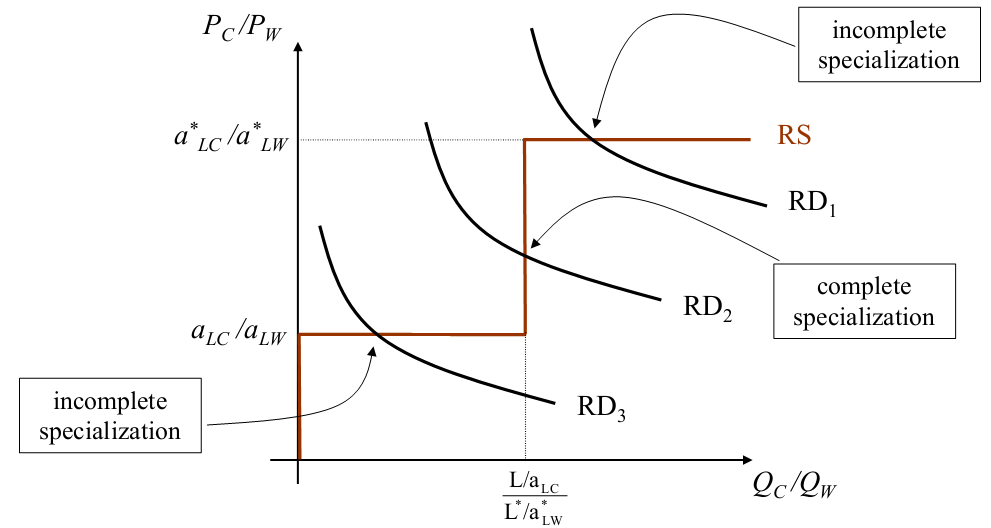
\includegraphics[width=11cm]{fig/ricardo/lec3-08}
\end{figure}


\end{frame}

\begin{frame}{A Numerical Example }


\begin{columns}[onlytextwidth]
\begin{column}{0.5\textwidth}
\begin{itemize}
\item Consider our previous example with England and Portugal, where $L$
=$L^{*}$ =100 
\item We can represent the “tech-nology matrix” as follows → 
\item Note that England has absolute advantage in both goods, but comparative
advantage in cloth: 5/10<4/6 
\item On the demand side, assume$U(D_{C},D_{W})=(D_{C})^{3/5}\cdot(D_{W})^{2/5}$
\end{itemize}

\end{column}
\begin{column}{0.5\textwidth}
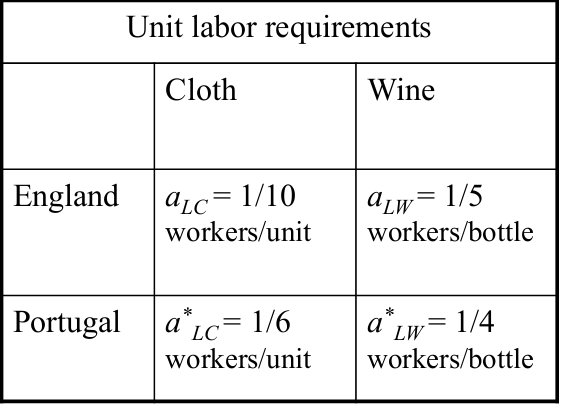
\includegraphics[width=\columnwidth]{fig/ricardo/lec3-09}
\end{column}
\end{columns}


\end{frame}

\begin{frame}{A Numerical Example (cont.) }


\begin{columns}[onlytextwidth]
\begin{column}{0.6\textwidth}
\begin{itemize}
\item According to related knowledge im Micro, relative demand is given
by
\[
\frac{D_{C}}{D_{W}}=\frac{3}{2}\centerdot\frac{1}{P_{C}/P_{W}}
\]

\item The relative supply curve is plotted on the right 
\[
\frac{L/a_{LC}}{L^{*}/a_{LC}^{*}}=\frac{100/(1/10)}{100/(1/4)}=2.5
\]

\item The equilibrium is:
\[
P_{C}/P_{W}=0.6
\]
\[
D_{C}/D_{W}=Q_{C}/Q_{W}=2.5
\]

\end{itemize}

\end{column}
\begin{column}{0.4\textwidth}
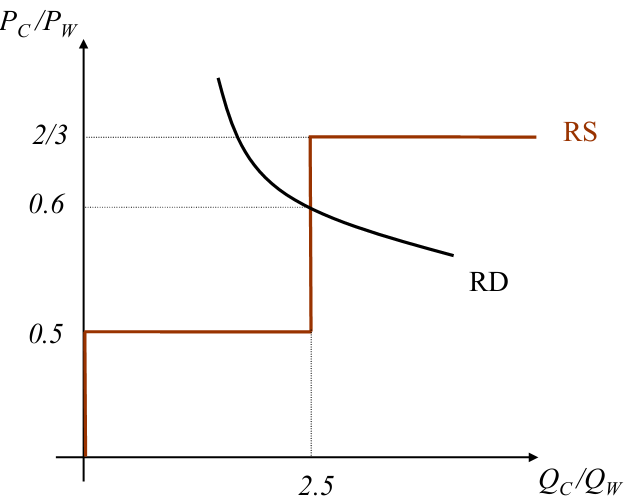
\includegraphics[width=\columnwidth]{fig/ricardo/lec3-10}
\end{column}
\end{columns}

\end{frame}

\begin{frame}{A Numerical Example (cont.) }

\begin{itemize}
\item We thus see that in equilibrium, England exports cloth and Portugal
exports wine
\item Furthermore, consistent with our suggested numbers: 

\begin{itemize}
\item England fully specializes in cloth and produces 1000 pieces of cloth 
\item Portugal fully specializes in wine and produces 400 bottles of wine 
\end{itemize}
\item This implies that income in England is $1000\cdot P_{C}$ , which
is spent on cloth ($P_{C}\cdot D_{C}$) and wine ($P_{W}\cdot D_{W}$
) 
\end{itemize}
\end{frame}

\begin{frame}{A Numerical Example (cont.)}

\begin{itemize}
\item From the demand side we also know that 
\[
2\text{·}P_{C}\text{·}D_{C}=3\text{·}P_{W}\text{·}D_{W}
\]

\item We thus have $(1+2/3)\cdot P_{C}\cdot D_{C}=1000\cdot P_{C}\rightarrow D_{C}=600$ 
\item Using $P_{C}/P_{W}=0.6$, we also have $D_{W}=240$ 
\item \textcolor{red}{Exercise:} show that $D_{C}^{*}=400$ and $D_{W}^{*}=160$ 
\item \textcolor{red}{Exercise:} show that in autarky, $D_{C}=600$ and
$D_{W}=200$ and $D_{C}^{*}=360$ and $D_{W}^{*}=160$ 
\end{itemize}
\end{frame}



\section{Gains From Trade}
\begin{frame}{Gains From Trade: Autarky}

\begin{itemize}
\item We can represent the autarkic equilibrium in each country as follows 
\end{itemize}

\begin{figure}
\begin{centering}
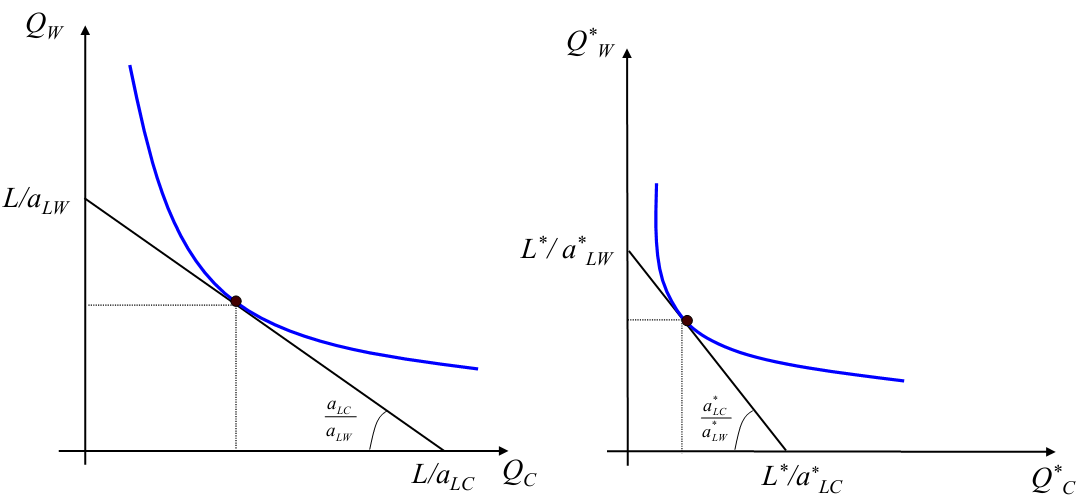
\includegraphics[width=12cm]{fig/ricardo/lec3-11}
\par\end{centering}

\end{figure}


\end{frame}

\begin{frame}{Gains From Trade: Graph }

\begin{itemize}
\item Free trade has an effect analogous to an expansion of the PPF 
\end{itemize}

\begin{figure}
\begin{centering}
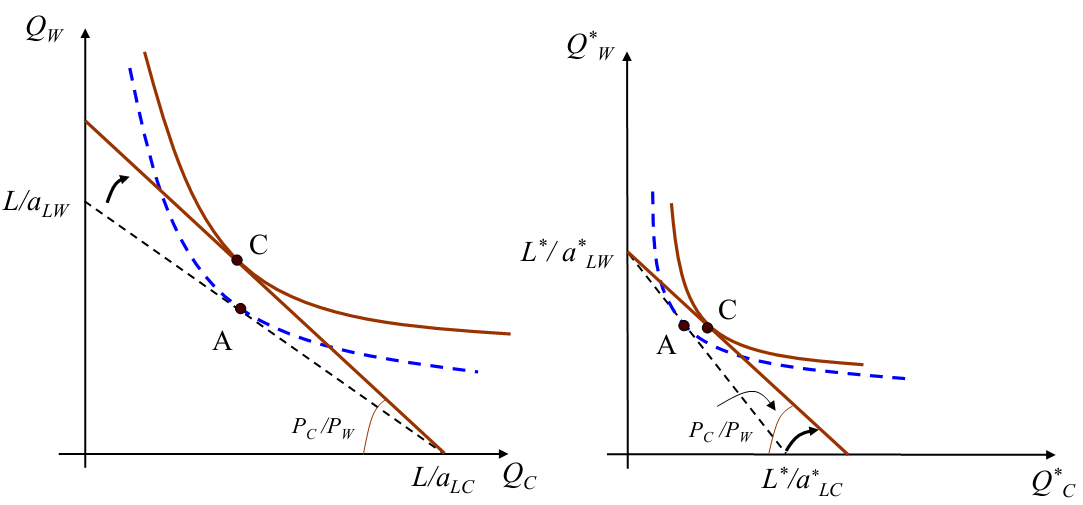
\includegraphics[width=12cm]{fig/ricardo/lec3-12}
\par\end{centering}

\end{figure}



\end{frame}

\begin{frame}{Dismantle Gains: Production(Division) vs. Consumption(exchange) Gains}


\begin{columns}[onlytextwidth]
\begin{column}{0.4\textwidth}
\begin{itemize}
\item There are actually two forces at play in shift from A to C 
\item Consumption gains from trade (A to B), as in Lecture 4 
\item Production gains from trade (B to C)
\end{itemize}

\end{column}
\begin{column}{0.6\textwidth}
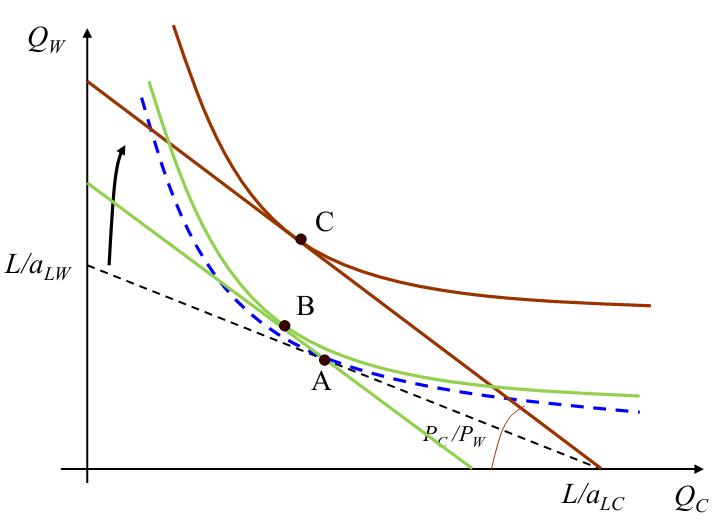
\includegraphics[width=\columnwidth]{fig/ricardo/lec3-13}
\end{column}
\end{columns}

\end{frame}

\begin{frame}{Distributional Effects (or lack thereof) }

\begin{itemize}
\item The Ricardian model is extremely simple in that: 

\begin{enumerate}
\item All workers are identical (or units of skill are perfect subst. 
\item Workers can costlessly transition between sectors 
\item All markets are perfectly competitive and all markets clear (hence,
no unemployment) 
\end{enumerate}
\item As a result, all workers gain from trade and there is no need for
redistribution 
\item The next two models we will present will feature distributional effects 
\end{itemize}
\end{frame}

\begin{frame}{Relative Wages}

\begin{itemize}
\item \textcolor{red}{Relative wages} are the wages of the domestic country
relative to the wages in the foreign country 
\item Although the Ricardian model predicts that goods’ prices equalize
across countries after trade, it does not predict that wages will
do the same 
\item Productivity (technological) differences determine wage differences
in the Ricardian model 

\begin{itemize}
\item A country with absolute advantage in producing a good will enjoy a
higher wage in that industry after trade.
\end{itemize}
\end{itemize}
 \begin{theorem}
 	比较优势决定分工(贸易)模式,绝对优势决定工资水平
 \end{theorem}
\end{frame}

\begin{frame}{证明}

\begin{itemize}
\item Notice that regardless of the type of equilibrium, Home workers produce
cloth and Foreign workers produce wine 
\item The wage at Home is thus equal to revenue per worker in cloth (remember
zero profits), and hence$w=P_{C}\cdot(1/a_{LC})$
\item The wage in Foreign equals revenue per worker in wine, so $w*=P_{W}\cdot(1/a_{LW}^{*})$
\item The relative wage of domestic workers is therefore 
\[
\frac{w}{w^{*}}=\frac{P_{C}}{P_{W}}\frac{a{}_{LW}^{*}}{a_{LC}}
\]

\end{itemize}
\end{frame}

\begin{frame}{证明 (cont.)}

\begin{itemize}
\item Remember that $P_{C}/P_{W}\ge a_{LC}/a_{LW}$ , and hence $w/w*\ge a_{LW}^{*}/a_{LW}$ 
\item Similarly, $P_{C}/P_{W}\le a_{LC}^{*}/a_{LW}^{*}$implies that $w/w*\le a_{LC}^{*}/a_{LC}$ 
\item Putting the pieces together we have that the relative wage lies between
the ratios of the two countries’ productivities in the two industries:
\[
a_{LC}^{*}/a_{LC}\text{\ensuremath{\ge}}w/w^{*}\text{\ensuremath{\ge}}a_{LW}^{*}/a_{LW}
\]

\end{itemize}
\end{frame}

\begin{frame}{Relative Wages (cont.) }


\[
a_{LC}^{*}/a_{LC}\text{\ensuremath{\ge}}w/w^{*}\text{\ensuremath{\ge}}a_{LW}^{*}/a_{LW}
\]

\begin{itemize}
\item If Home has absolute advantage in both industries, then $w>w*$ 

\begin{itemize}
\item In our recurrent example, we have that $w/w*=1.5$
\end{itemize}
\item With complete specialization, $w/w*$ will fall strictly between the
bounds (each countries has a cost advantage in one good) 
\item When both countries produce the same good, relative wages are given
by the ratio of productivities in that good (absolute advantage determines
wages) 
\end{itemize}
\end{frame}

\begin{frame}{Preliminary Empirical Evidence }


\begin{columns}[onlytextwidth]
\begin{column}{0.5\textwidth}
\begin{itemize}
\item In the Ricardian model, relative wages reflect the relative productivities
of the two countries 
\item Some argue that low-wage countries pay low wages despite growing productivity,
putting high -wage countries at a cost disadvantage 
\item What does the evidence suggest? 

\end{itemize}

\end{column}
\begin{column}{0.5\textwidth}
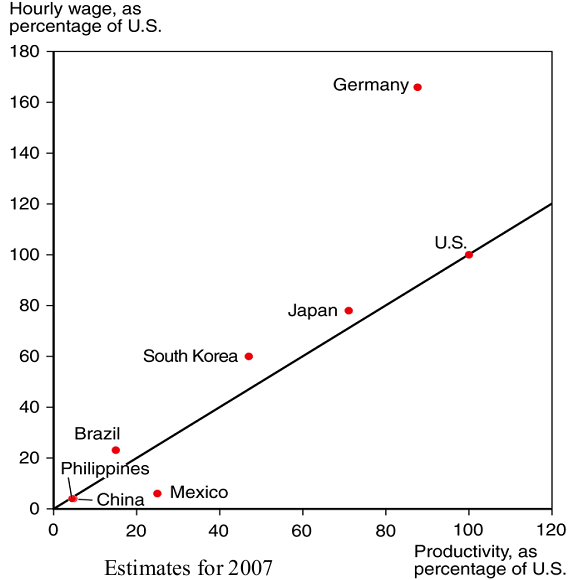
\includegraphics[width=0.8\columnwidth]{fig/ricardo/lec3-14}
\end{column}
\end{columns}
\pause
\structure{\textbf{结论}:生产率的提升会反映在工资增长中}

\end{frame}

\begin{frame}{Misconceptions}

\begin{itemize}
\item We have dispelled the following misconceptions \end{itemize}
\begin{enumerate}
\item Free trade can be beneficial only if a country is strong enough to
stand up to foreign competition 

\begin{itemize}
\item gains from trade are related to comparative advantage 
\end{itemize}
\item Free trade with countries that pay low wages hurts high- wage countries
and is unfair 

\begin{itemize}
\item Free trade will lead to the dislocation of some workers, but these
workers can (in principle) transition to another sector that leaves
them with higher real income, due to lower relative price of imported
good 
\item Bastiat’s \textbf{\textcolor{blue}{\uline{“\href{http://bastiat.org/en/petition.html}{Petition of the Candle Makers}}}}” 
\end{itemize}
\item Free trade exploits less productive countries 

\begin{itemize}
\item On welfare grounds they are better off 
\item What about labor standards and so on? Key question: what is the counterfactual? 
\end{itemize}
\end{enumerate}
\end{frame}

\begin{frame}{Frédéric Bastiat (巴师夏,1801 -1850) }


\begin{figure}


\begin{centering}
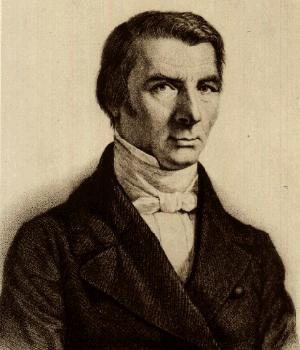
\includegraphics[width=6cm]{fig/ricardo/lec3-15}\protect\caption{Economic Sophisms, 1845 }

\par\end{centering}

\end{figure}

\end{frame}

\begin{frame}{Petition of the Candle Makers}


“We are suffering from the \textbf{\textcolor{green}{ruinous competition}}
of a rival who apparently works under conditions so far superior to
our own for the production of light that he is \textbf{\textcolor{green}{flooding
the domestic market}} with it at an \textbf{\textcolor{green}{incredibly
low price}} {[}…{]} This rival, which is none other than the sun,
is waging war on us so mercilessly we suspect he is being stirred
up against us by perfidious Albion (excellent diplomacy nowadays!),
particularly because he has for that haughty island a respect that
he does not show for us.” 


\end{frame}

\begin{frame}{Petition of the Candle Makers}


“We ask you to be so good as to pass a law requiring the closing of
all windows, dormers, skylights, inside and outside shutters, curtains,
casements, bull's- eyes, deadlights, and blinds — in short, all openings,
holes, chinks, and fissures through which the light of the sun is
wont to enter houses, to the detriment of the fair industries with
which, we are proud to say, we have endowed the country, a country
that cannot, without betraying ingratitude, abandon us today to \textbf{\textcolor{green}{so
unequal a combat }}.” 
\end{frame}



\section{Extensions of the Ricardo Model(选修)}


\subsection{Introducing Non-Traded Goods}
\begin{frame}{Introducing Non -Traded Goods }

\begin{itemize}
\item Imagine now that there is a third good, “haircuts”, that can be produced
both at Home and in Foreign, but that is not tradable 
\item A haircut requires $a_{LH}$ units of labor at Home and $a{}_{LH}^{*}$
in Foreign 
\item Suppose that preferences are such that haircuts are always produced
in both countries 
\end{itemize}
\end{frame}

\begin{frame}{Equilibrium with Non -Traded Goods}

\begin{itemize}
\item Zero profits imply $P_{H}=wa_{LH}$and$P{}_{H}^{*}=w^{*}a_{LH}^{*}$
\item Now assume further that productivity differences in the production
of nontradables are small, so $a$$_{LH}=a_{LH}^{*}$
\item It then follows that $P_{H}/P_{H}^{*}=w/w^{*}$
\item So countries with higher wages will tend to feature higher prices
for “nontradables” 
\item And they will also feature higher aggregate price levels (since $P_{C}=P_{C}^{*}$
and $P_{W}=P_{W}^{*}$)
\end{itemize}
\end{frame}

\begin{frame}{Balassa-Samuelson Effect}

\begin{itemize}
\item How do non-traded goods affect the determination of world equilibrium?
How is $w/w*$ determined? 
\item The analysis is more complicated, but it continues to be the case
that relative wages are higher in countries with higher productivity
levels in the production of tradable goods 
\item If $U(D_{C},D_{W},D_{H})=(D_{C})^{a}\cdot(D_{W})^{b}\cdot(D_{H})^{1-a-b}$
, the solution of the model is actually almost identical to that of
the model without non -traded goods 
\item \textbf{\textcolor{green}{Balassa- Samuelson Effect:}} consumer price
levels in wealthier countries are systematically higher than in poorer
ones because productivity levels vary more by country in the traded
-good sectors than in other sectors 
\end{itemize}
\end{frame}

\begin{frame}{Some Evidence }


\begin{figure}
\begin{centering}
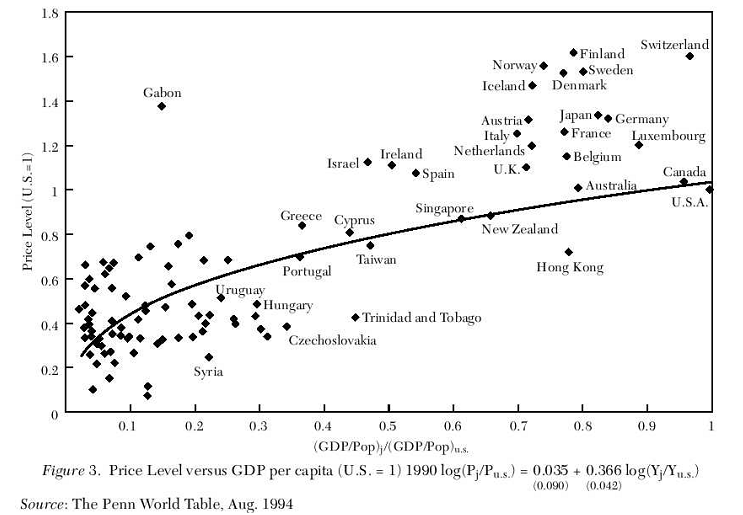
\includegraphics[width=9cm]{fig/ricardo/lec3-16}
\par\end{centering}

\end{figure}

\end{frame}

\begin{frame}{Some Implications }


\begin{figure}


\begin{centering}
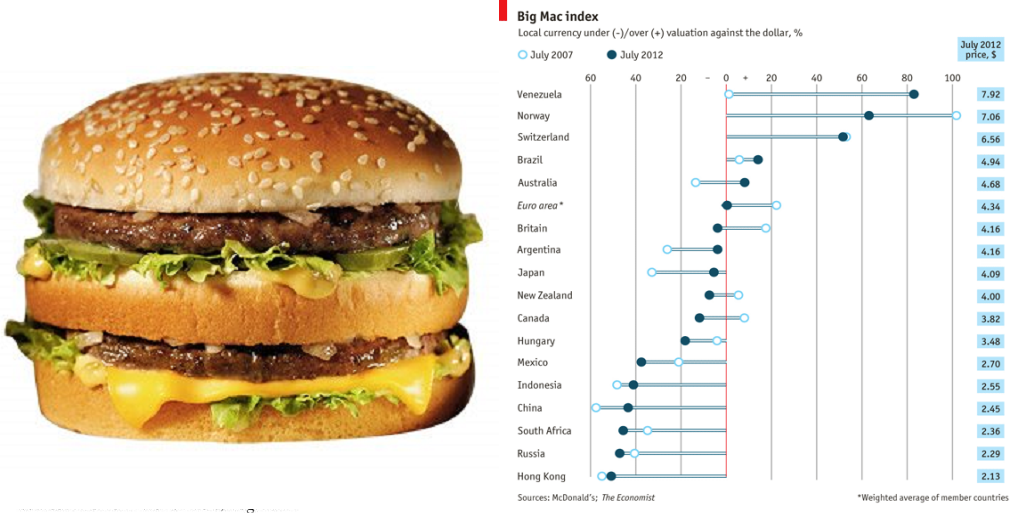
\includegraphics[width=12cm]{fig/ricardo/lec3-17}
\par\end{centering}

\end{figure}

\end{frame}

\begin{frame}{What’s Behind the Index? }


\begin{figure}
\begin{centering}
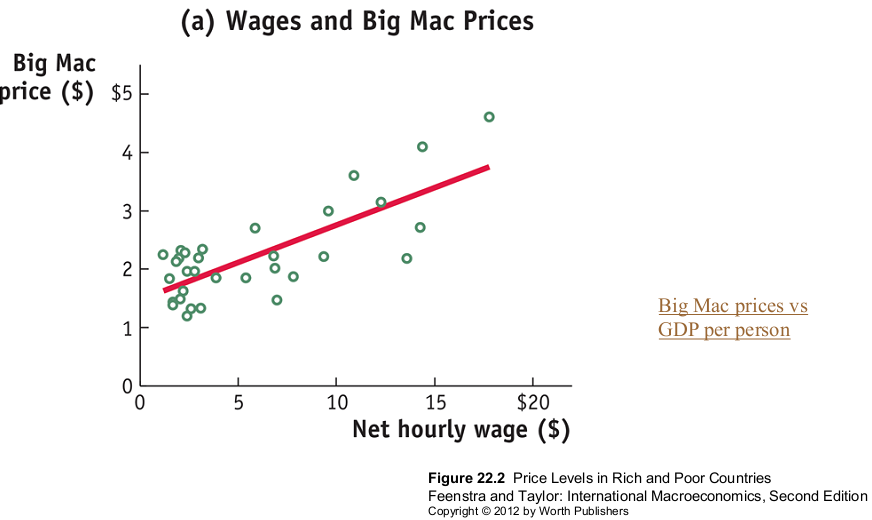
\includegraphics[width=11cm]{fig/ricardo/lec3-18}
\par\end{centering}

\end{figure}

\end{frame}

\begin{frame}{Transportation Costs }

\begin{itemize}
\item Now assume that it costs $t\%$ of the price of a good to ship one
unit from one country to the other 
\item If good $i$ is produced in Home, then it sells for $p_{i}=wa_{Li}$
in Home and can be imported at price $p_{i}^{*}=(1+t)p_{i}$ in Foreign
(to cover transport costs) 
\item If $w^{*}a_{Li}^{*}<(1+t)wa_{Li}$ then Foreign would not import the
good, but produce it instead (even if $w^{*}a_{Li}^{*}>wa_{Li}$) 
\item Similarly, if $wa$$_{Li}<(1+t)w^{*}a_{Li}^{*}$ then Home would not
import the good, but produce it instead (even if $w^{*}a_{Li}^{*}<wa_{Li}$
) 
\item The higher the transport cost $t$, the more non -traded goods there
will be 
\end{itemize}
\end{frame}



\subsection{Introducing Multiple Goods }
\begin{frame}{Introducing Multiple Goods }

\begin{itemize}
\item Suppose now there are N tradable goods, indexed by $i=1,2,\ldots,N$. 
\item Home’s unit labor requirement for good i is $a{}_{Li}$ , Foreign’s
is $a_{Li}^{*}$ 
\item Goods will be produced wherever it is cheaper to produce them 

\begin{itemize}
\item If $wa_{L1}<w^{*}a_{L1}^{*}$ then only Home country will produce
good 1, since total wage payments are lower at Home 
\end{itemize}
\end{itemize}
\end{frame}

\begin{frame}{Pattern of Trade with Multiple Goods}

\begin{itemize}
\item Suppose goods are ranked such that $a_{Li}^{*}/a_{Li}$ is increasing
in $i$ 

\begin{itemize}
\item the higher $i$, the larger the comparative advantage of Home 
\end{itemize}
\item Then we will have 
\[
a_{L1}^{*}/a_{L1}<\text{…}<a_{LI}^{*}/a_{LI}\text{\ensuremath{\le}}w/w^{*}\text{\ensuremath{\le}}a_{LI+1}^{*}/a_{LI+1}<\text{…}<a_{LN}^{*}/a_{LN}
\]

\item And Home produces all the goods with index$I+1$ or higher, and possibly
also good$I$
\end{itemize}
\end{frame}

\begin{frame}{Introducing Multiple Goods (cont.) }


\begin{columns}[onlytextwidth]
\begin{column}{0.5\textwidth}
\begin{itemize}
\item How is the relative wage $w/w*$determined? 

\begin{itemize}
\item Relative supply and relative (derived) demand for labor are equalized 
\end{itemize}
\item Suppose that the relative supply is exogenous and given by $L/L*$ 
\item The relative (derived) demand for Home labor services falls when $w/w*$
rises as Home becomes the least -cost producer of less and less goods 
\item Consider case of two goods 
\end{itemize}

\end{column}
\begin{column}{0.5\textwidth}
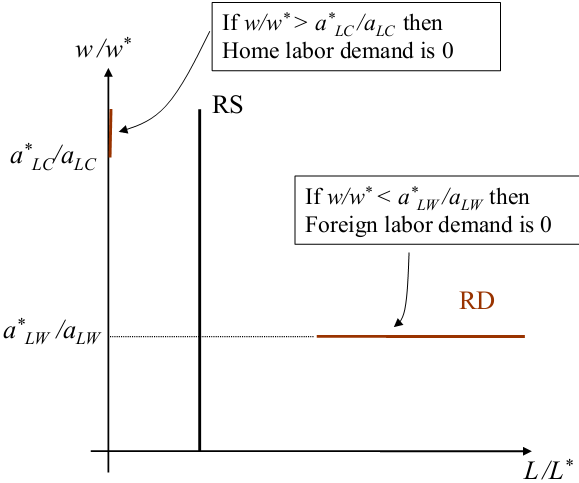
\includegraphics[width=\columnwidth]{fig/ricardo/lec3-19}
\end{column}
\end{columns}

\end{frame}

\begin{frame}{Introducing Multiple Goods (cont.) }


\begin{columns}[onlytextwidth]
\begin{column}{0.5\textwidth}
\begin{itemize}
\item Note that when $L/L*$ is low, Foreign will produce both goods: 
\[
w/w^{*}=a{}_{LC}^{*}/a_{LC}
\]

\item Conversely, when L/L{*} is high, Home will produce both goods 
\[
w/w^{*}=a{}_{LW}^{*}/a_{LW}
\]

\item With complete specialization: 
\[
w/w^{*}=(P_{C}/P_{W})\text{·}(a_{LW}^{*}/a_{LC})
\]

\end{itemize}

\end{column}
\begin{column}{0.5\textwidth}
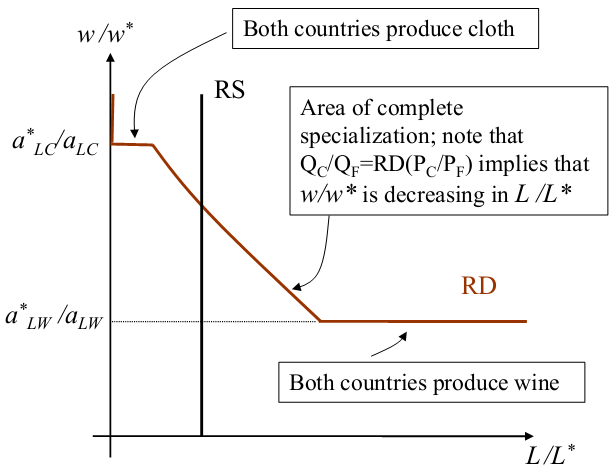
\includegraphics[width=\columnwidth]{fig/ricardo/lec3-20}
\end{column}
\end{columns}


\end{frame}

\begin{frame}{Introducing Multiple Goods (cont.) }


\begin{columns}[onlytextwidth]
\begin{column}{0.6\textwidth}
\begin{itemize}
\item With multiple goods, the graph is analogous 
\item Note that Home and Foreign produce \textbf{\textcolor{green}{at most
one good in common ! }}
\item This strong implication however crucially relies on the absence of
transportation costs (see next slide) 
\item All countries gain from trade as long as they import a good they don’t
produce
\end{itemize}

\end{column}
\begin{column}{0.4\textwidth}
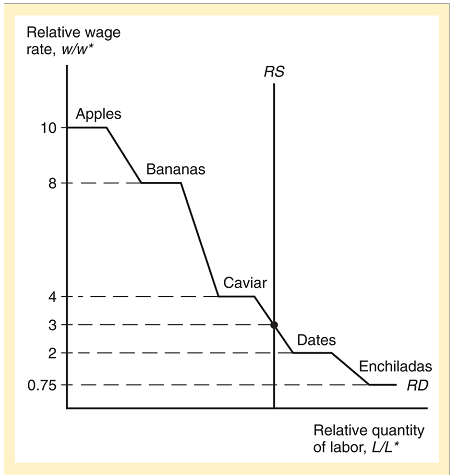
\includegraphics[width=0.8\columnwidth]{fig/ricardo/lec3-21}
\end{column}
\end{columns}

\end{frame}



\section{Further Empirical Evidence}
\begin{frame}{Empirical Evidence: Balassa (1963) }


\begin{columns}[onlytextwidth]
\begin{column}{0.6\textwidth}
\begin{itemize}
\item Do countries export those goods in which their productivity is relatively
high? 
\item The ratio of US to British exports in 1951 (the year of Lecture 1’s
video!) compared to the ratio of US to British labor productivity
in 26 manufacturing industries suggests “yes” 
\item At this time the US had an absolute advantage in all 26 industries,
yet the ratio of exports was low in the least productive sectors of
the US 
\end{itemize}

\end{column}
\begin{column}{0.4\textwidth}
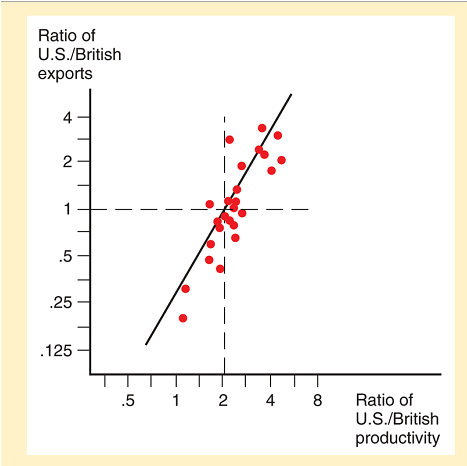
\includegraphics[width=\columnwidth]{fig/ricardo/lec3-22}
\end{column}
\end{columns}

\end{frame}

\begin{frame}{Measurement of CA: Revealed comparative advantage}

\begin{itemize}
\item The current resurgence of interest in industrial policy sometimes
confronts trade economists with demands to identify sectors of comparative
advantage. However, this is not a straightforward task. 
\item The traditional measure is the revealed comparative advantage (RCA)
index\textcolor{blue}{{} (Balassa, 1965)}. It is a ratio of product
$k$’s share in country $i$’s exports to its share in world trade.
Formally
\[
RCA_{k}^{i}=\frac{X_{k}^{i}/X^{i}}{X_{k}/X}
\]

\item A disadvantage of the RCA index is that it is asymmetric.
\item Laursen (2000) normalized RCA index, say NRCA
\[
NRCA_{k}^{i}=\frac{RCA_{k}^{i}-1}{RCA_{k}^{i}+1}
\]

\item the lower (–1) and upper (+1) bounds are now symmetric
\end{itemize}
\end{frame}

\begin{frame}{Conceptual Problem and Ingenious Test }

\begin{itemize}
\item Theory predicts that countries specialize, so how would one observe
the productivity of a country in a set of goods it does not produce? 
\item Ingenious test suggested by Costinot and Donaldson (2012) : agronomists
at FAO have estimated the productivity of a given parcel of land,
were it to be used to grow any one of a set of crops 
\item Their empirical results show that the output levels predicted by Ricardo’s
theory of comparative advantage agree reasonably well with actual
data on worldwide agricultural production 
\end{itemize}
\end{frame}

\begin{frame}{Ingenious Test }


\begin{figure}


\centering{}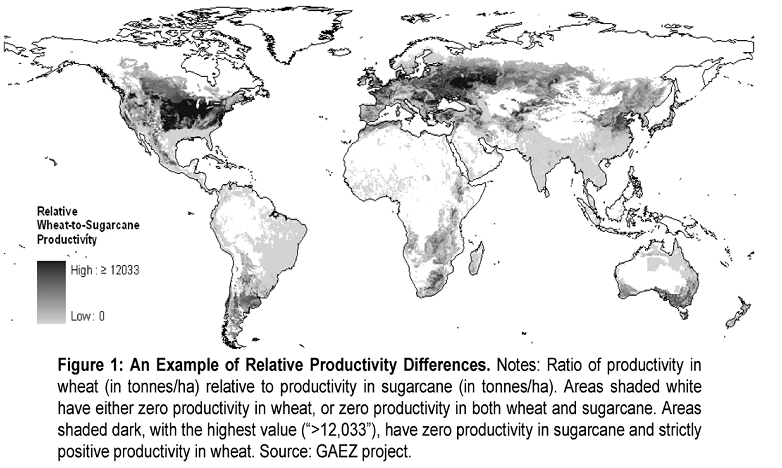
\includegraphics[width=11cm]{fig/ricardo/lec3-23}
\end{figure}

\end{frame}

\begin{frame}{}


\begin{figure}


\begin{centering}
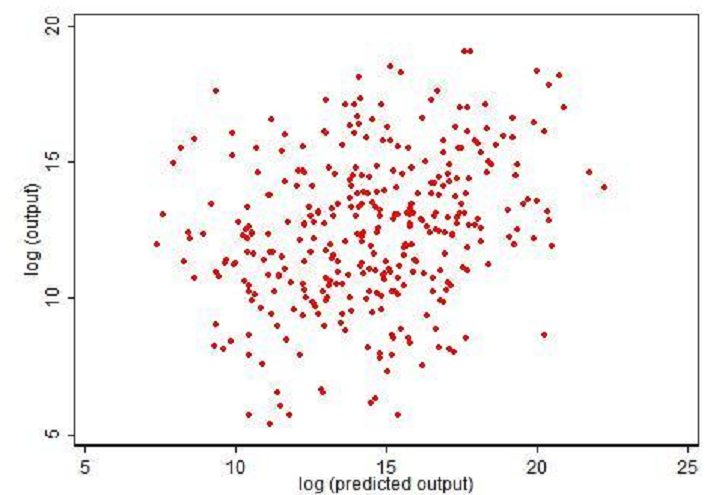
\includegraphics[width=11cm]{fig/ricardo/lec3-24}
\par\end{centering}

\end{figure}

\end{frame}

\begin{frame}{Limitations of Ricardian Model}

\begin{itemize}
\item The model ignores distributional issues, without which it is hard
to make sense of protectionism 
\item It ignores the role of other factor endowments in determining trade
flows across countries 
\item It ignores the role of scale economies in determining trade flows
across countries 
\end{itemize}
\end{frame}

\begin{frame}{Agenda for Next Week}

\begin{itemize}
\item Gains and Losses from Trade in the Specific-Factors Model

\begin{itemize}
\item Specific Factors Model (I): Motivation. Model Assumptions and Autarky
Equilibrium 
\item Specific Factors Model (II): Trade Equilibrium, Distributional Conflict
and Primer on Trade Policy 
\item Specific Factors Model (III): An Application to the Study of Migration 
\end{itemize}
\item Readings: 

\begin{itemize}
\item K-O-M Chapter 3 
\item F-T Chapter 3

\end{itemize}
\end{itemize}
\end{frame}

\end{document}



\end{document}